% !TEX root = ../thesis.tex
\chapter{Backgroud}
\label{chap:Utilized Tools}

\section{Openstack}
\label{sec:openstack}
\subsection{Overview}
OpenStack\cite{OpenStackwebsite} is an open-source cloud toolkit consisting of a series of interrelated projects that control pools of processing, storage and networking resources in a datacenter.
This project, started in 2010, aims to behave as a datacenter operating system or cloud OS.
As a traditional operating system, a cloud operating system has the main purpose to export an abstraction of the physical hardware but, instead of piloting directly the integrated circuits via drivers as in the single server case, it has the ability to interface itself with an arbitrary number of agents resident over the hypervisor - or virtual machine monitor (VMM) - of each physical server's operating system, in other words it behaves as a manager of hypervisors.
Cloud operating systems simplify the management of a datacenter in which virtual machines are heavily utilized. In fact, they provide a level of abstraction in which all the physical servers are seen and can be managed from a single point.

The OpenStack project aims to provide a centralized interface to be used by datacenter administrators, giving them an overview about resources availability, usage and status and therefore putting them in the position to plan maintenance or provision hardware resizing in order to keep up with the demanded computational power.
Being a commercial product and not only a proof of concept, OpenStack is also engineered to allow the coexistence of administrators and normal users, the firsts are in charge of monitoring the resources availability and manage the infrastructure of the datacenter, providing to the seconds the possibility to instantiate virtual machines and interconnecting them without worrying about configuring the physical infrastructure and the actually available resources.
Normal user is a general term that will refer to an actor that does not have administrative privileges (i.e., he does not have full control over the system); in the case of OpenStack, a user can correspond to either a single person, a department in a company or even to an entire firm that decides to rely on an external infrastructure in where to deploy the virtual servers that provide the services needed for business.
Of course this automation and level of abstraction come at a price which is affordable without any problem in a datacenter environment; on the other hand, in the case of very small amount of physical machines, the overhead is not negligible even if not exaggerate, as can be seen in table~\ref{tbl:components_resource_usage2} (note that the data are taken when the system is at operating speed and many of the OpenStack components works with a caching system). % and further inspected later.
Let's say that in general, when the number of equipments exceeds the few units and the virtual machines creation and deletion volume is high enough to overload the amount of requests that administrators can keep up with, the effort to install the OpenStack system will be well rewarded.

\subsection{General design architecture}
OpenStack has been developed having in mind five guidelines, which are:
\begin{itemize}
    \item Component based architecture, to quickly add new behaviors.
    \item Highly capable of easily scale up/down.
    \item Fault tolerant, isolated processes avoid cascading failures.
    \item Recoverable, failures should be easy to diagnose, debug, and rectify.
    \item Open standards, be a reference implementation for a community-driven API.
\end{itemize}
As mentioned above, OpenStack is not a single project but a pool of independent modules that communicate together, each one in charge of providing one or more functionalities (e.g., computing and network management, authentication, etc).
Modularity has two main benefits: the first one is to permit datacenter administrators to choose what features they want and what they do not, enabling the possibility to offer users different typologies of service; the second advantage is the interchangeability of modules that are designed for the same purpose (e.g., network management) so that an administrator can pick the module that suits the best or even write one by himself from scratch.
The majority of modules are, in turn, split into submodules and designed to allow plugging in special purpose add-ons written to accomplish specific tasks or made the module behave in a certain desired way.

\subsection{Physical architecture}
The deployment of OpenStack requires a total amount of three logically separated entities that can be remapped into one or more physical machines.
These three entities are generally referred as the following:
\begin{itemize}
    \item \textbf{Controller node}.
    \item \textbf{Compute node}.
    \item \textbf{Network node}.
\end{itemize}

In the \textbf{Controller node} resides a set of supporting services, basic (or core) components and a series of optional features.
Supporting services are not properly OpenStack components but are necessary for its operations; two of these components are the database management system (e.g., MySQL\cite{mysql}) for persistent storage and the message broker (e.g., RabbitMQ\cite{rabbitmq}) for modules intercommunication. Having them in the controller node is not mandatory but since the major share of requests to this components comes from services also resident in the control node, delays due to the network are eliminated.
Basic components are all those OpenStack modules that provide the very basic functionalities and that will become the "brain" in charge of managing the whole infrastructure.
In addition, in the controller node can be installed optional components that are not crucial but offer useful functionalities such as Ceilometer. Ceilometer is the OpenStack telemetry service that tracks resources usage aggregated by user, giving the possibility to manage billing in case of a datacenter offered as a service.
Another optional component is the orchestrator known as Heat that is in charge of communicating with both the network and the compute manager.
The controller node needs to communicate directly with all the other nodes (via a management interface) to dispatch commands and receive updates from them as depicted in Figure~\ref{fig:os_cloud} and further detailed in Figure~\ref{fig:OSarchitecture}.

The \textbf{Compute node} is in charge of actually hosting the virtual machines. This node is a single physical server and, if we consider the controller node as the brain of OpenStack, this compute node can be seen as the muscles. Since all the control services are hosted in the controller node, the amount of software required to be installed in the compute node is minimal, saving computing resources for the virtual instances that will be deployed on it. The only pieces of code required are an agent that communicates with the local hypervisor and - optionally - another agent that takes care of accepting particular commands to provide traffic isolation between users. In addition, in case of usage of optional services that require a distributed agent to retrieve statistics, also these agents run in the compute node.
Compute nodes are connected to the controller node in order to receive instructions, and have a separated network interface, referenced as \texttt{"instance tunnel"} in Figure~\ref{fig:OSarchitecture}, to communicate with each other, permitting to users' VMs to exchange traffic.
An edge of this network of Compute nodes there is the Network node.

The \textbf{Network node} is the border between the OpenStack domain and the outside world; in particular, is in charge of being the only node that has the capability to connect to the external network and let VMs traffic in and out to the Internet. It is also connected to the Controller node to receive commands. VMs are not instantiated in this frontier component, but it runs agents that will be in charge of providing basilar network services such as network address translation (NAT), ip assignation (DHCP) and privacy policies via a firewall.
\begin{table}[h]
\begin{tabular}{l|l|}
\cline{2-2}
                                                          & RAM {[}MB{]} \\ \hline
\multicolumn{1}{|l|}{\textbf{Controller node - full installation}} & 2100         \\ \hline
\multicolumn{1}{|l|}{\textbf{Controller node - minimal installation}}                                   & 1500         \\ \hline
\multicolumn{1}{|l|}{\textbf{Compute node}}                                   & 590          \\ \hline
\multicolumn{1}{|l|}{\textbf{Network node}}                                   & 250          \\ \hline
\end{tabular}
\centering
\caption{OpenStack nodes - resource analysis.}
\label{tbl:components_resource_usage2}
\end{table}

\label{a:br_section}
In the classic architecture of an OpenStack domain, each compute node have two virtual switches that can either be linux bridges, openvswitches\cite{ovswebsite} or xDPd\cite{xdpdwebsite}: one for attaching the VMs (generally called br-int) and the other (referred as br-net or br-tun) to create virtual tunnels with the other compute nodes, establishing a full mesh network that will carry packets from one server to another, thus making the intermediate network infrastructure completely transparent. The Network node, in addition to these two bridges, has another one (usually referred as br-ex) to which is bridged the physical network interface card (NIC) that has access to the Internet. As said before, the network node does not host virtual instances but instead it hosts network services; these services are attached to the br-int.
The br-int and the br-ex in the Network node are not linked in any way so that neither traffic can leave the inside of the datacenter, nor outside packets can enter the private network, unless a specific service (a router) is deployed and linked with two virtual interfaces, one connected to each of the two software switches.

Logical schemes for better understanding the complex architecture is provided in Figure~\ref{fig:os_cloud},~\ref{fig:OSarchitecture} and~\ref{fig:os_coud_with_br}, more details of the depicted services are available in section \ref{a:main_components}.
\begin{figure}[h]
	\centering
	% left bottom right top
	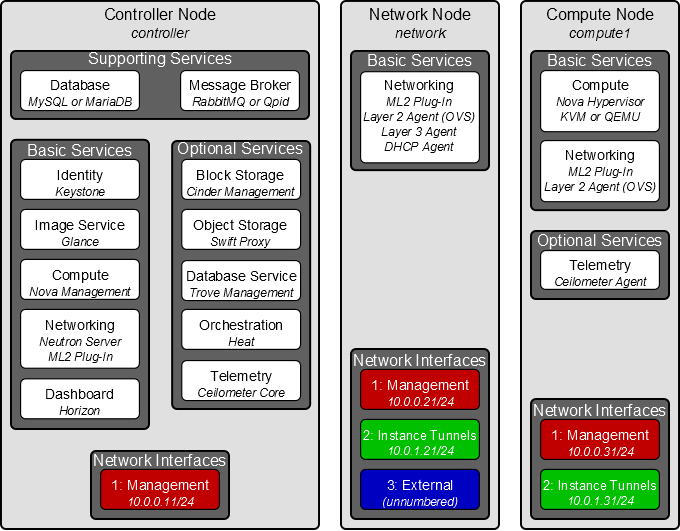
\includegraphics[clip= true, width=0.8 \columnwidth]{images/openstack_nodes.png}
	\caption{OpenStack logical nodes - services and interfaces.}
	\label{fig:OSarchitecture}
\end{figure}
\begin{figure}[h]
	\centering
	% left bottom right top
	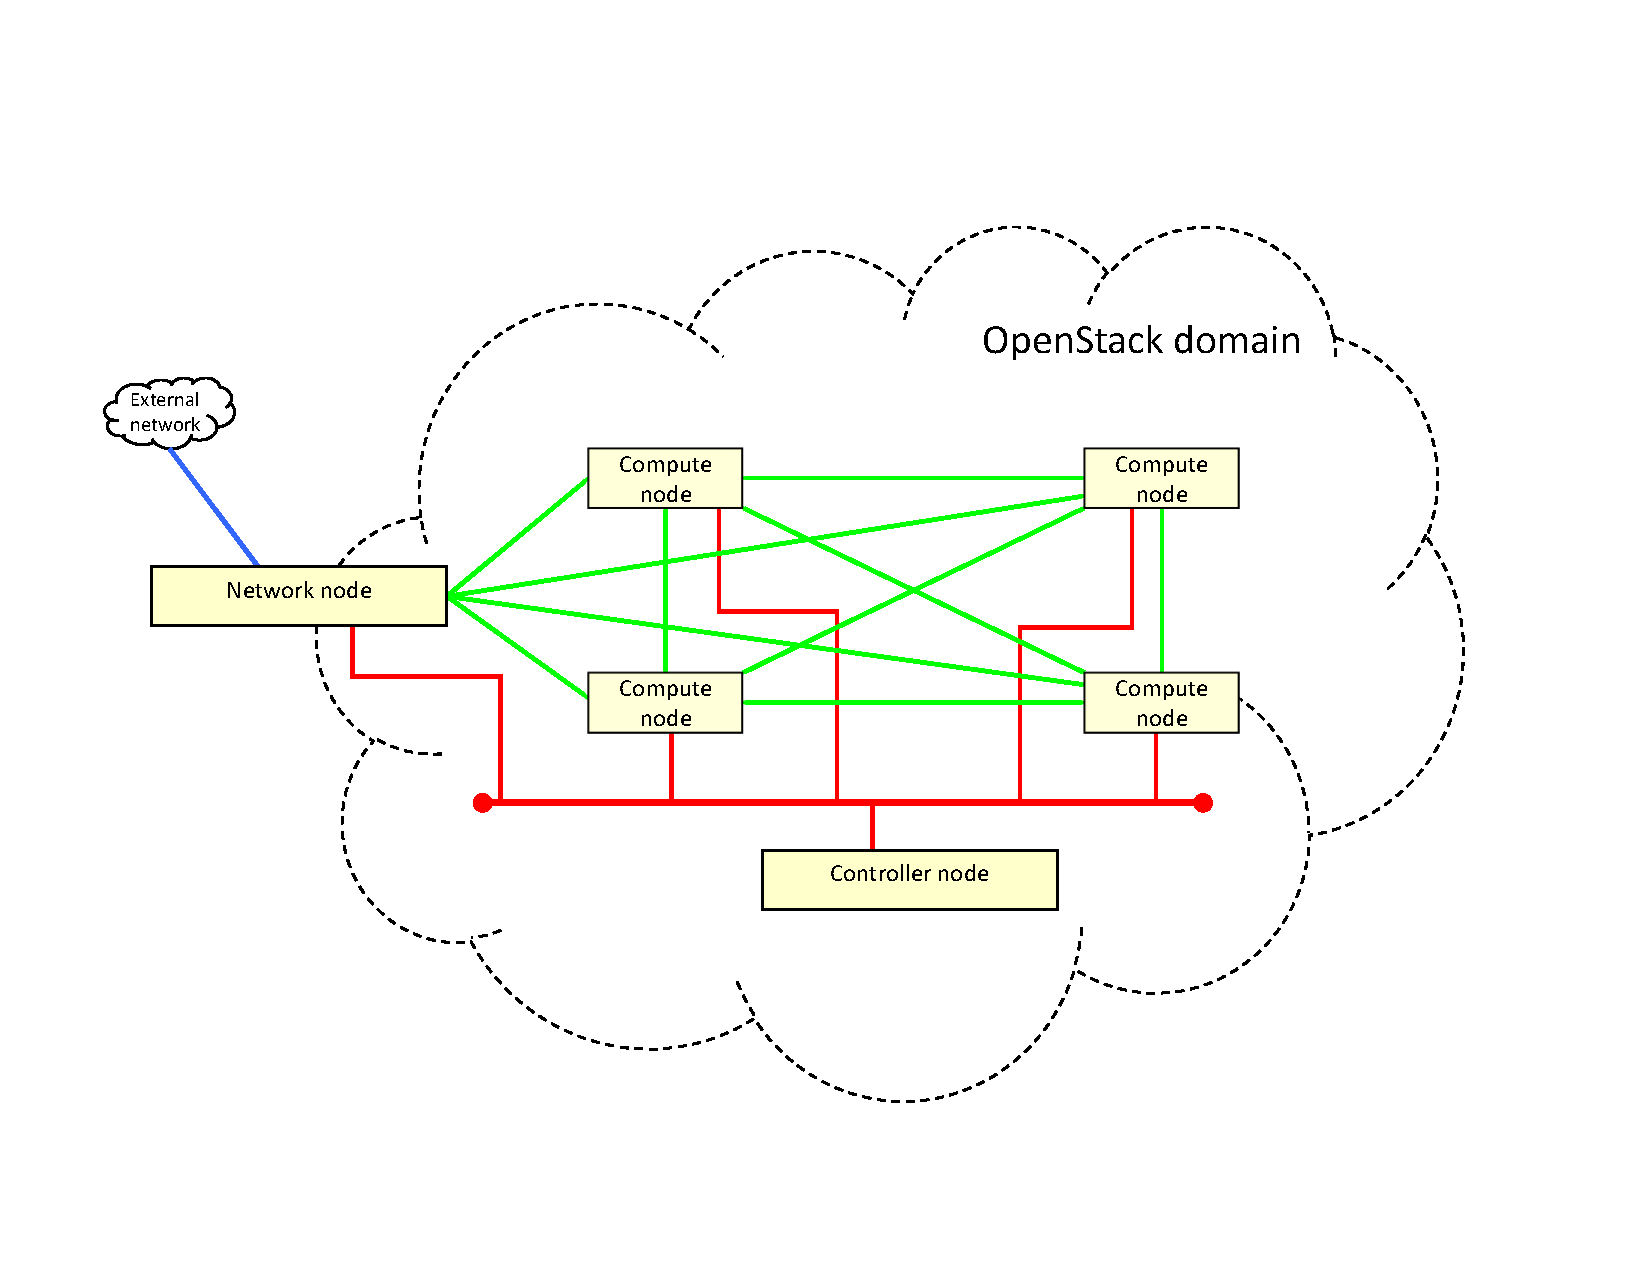
\includegraphics[clip= true, width= \columnwidth, trim=0cm 1cm 0cm 3cm]{images/os_cloud.pdf}
	\caption{OpenStack domain - Nodes interconnections.}
	\label{fig:os_cloud}
\end{figure}
\begin{figure}[h]
	\centering
	% left bottom right top
	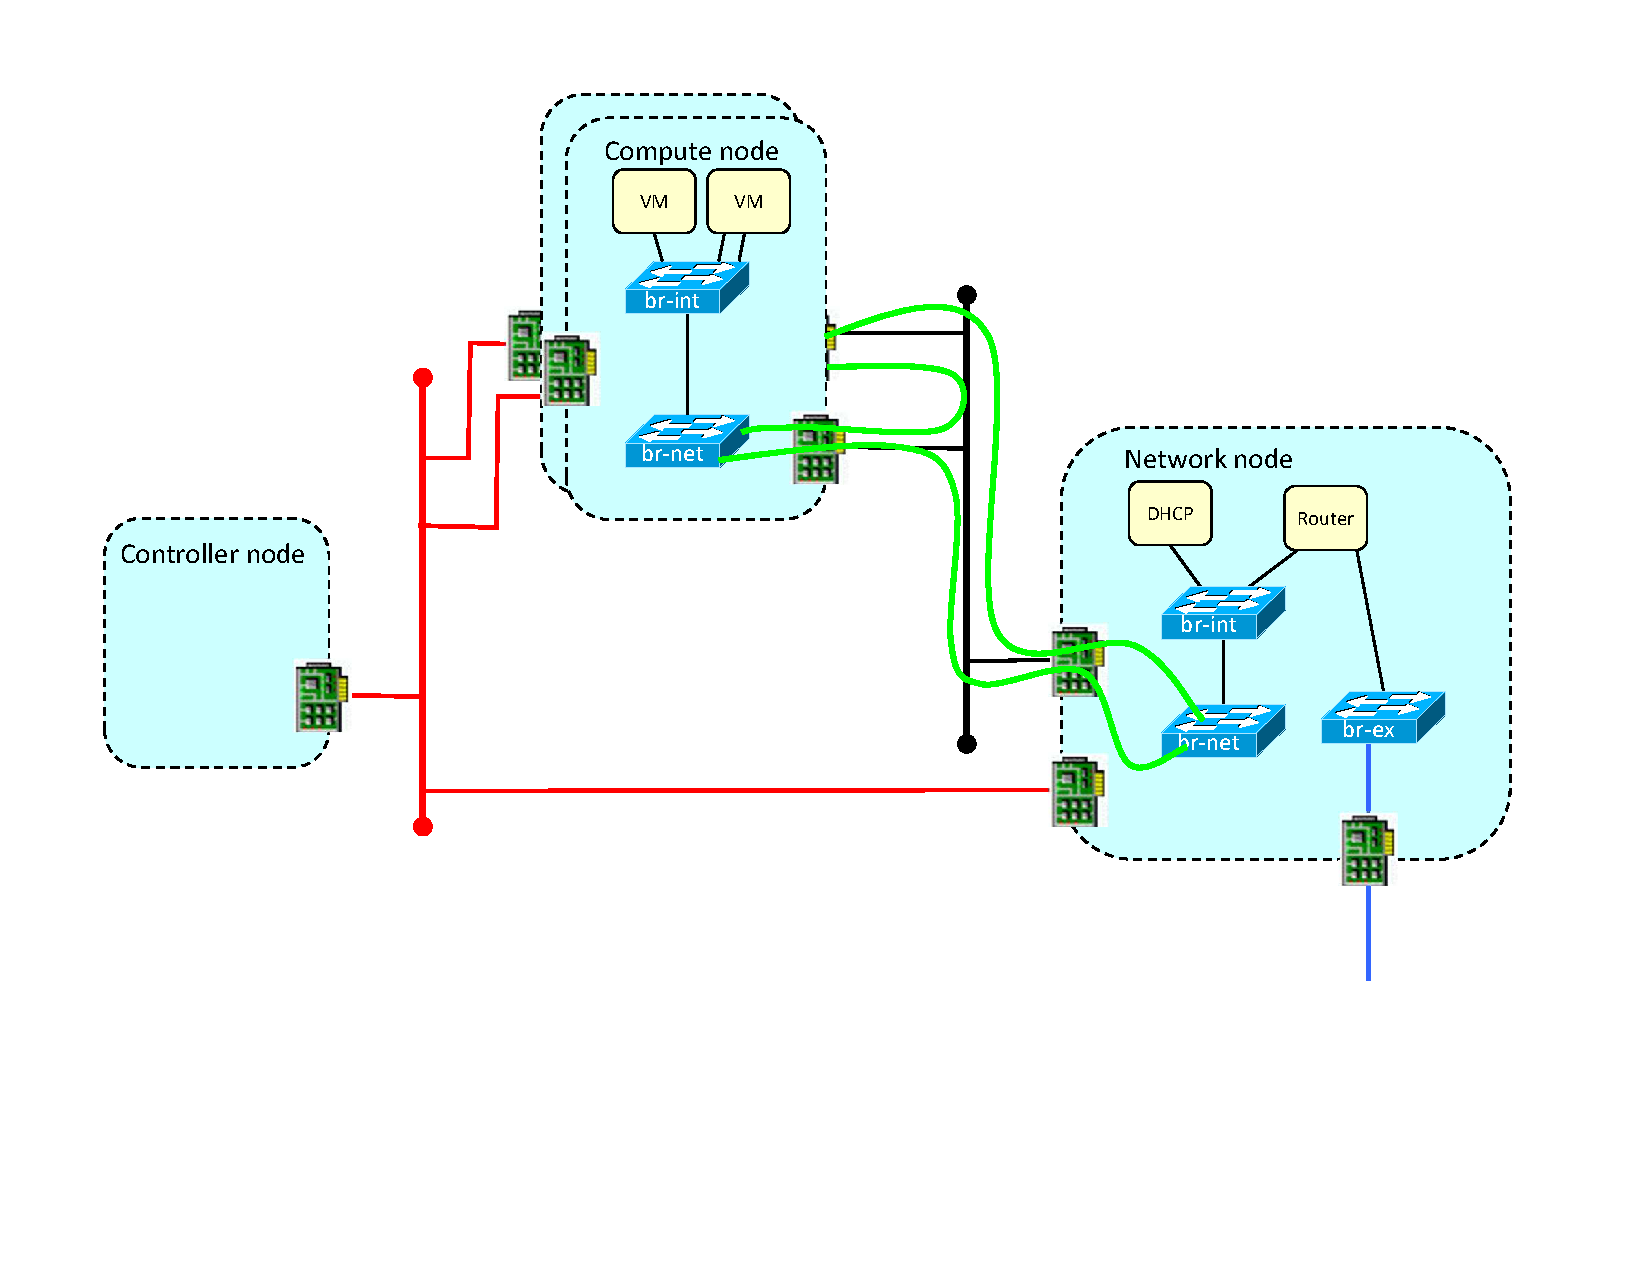
\includegraphics[clip= true, width= \columnwidth, trim=0cm 3cm 0cm 0cm]{images/os_cloud_with_br.pdf}
	\caption{OpenStack domain - Nodes interconnections in detail.}
	\label{fig:os_coud_with_br}
\end{figure}

%aggregation of logical entities
The logical architecture just described, depending on the size and computing power of the datacenter, can be remapped in various ways; in particular, the three entities can be aggregated as the administrator likes at installation time: a common deployment is to devolve one server serving as controller node and one as a network node, plus a number of compute nodes. However, in case of a very small datacenter in which there are just some physical machines nodes can be collapsed, even, OpenStack can be used to manage just one server; in this particular case one single machine will have all the three entities at the same time. Evidently the last example is a critical situation in which the introduced overhead is really influencing the performance, therefore this kind of configuration is useful only for developing and testing purposes.

\subsection{Main components}
\label{a:main_components}
OpenStack modules (called services in the follows) communicate together either via RESTful API or via a message broker server and may have the need to query a database. Additionally, in case of a datacenter as a service provided to external users, OpenStack offers a web interface - the Horizon dashboard - that requires a web server in order to serve users' requests.
These three additional services are not part of the core components of OpenStack but, based on the standard configuration, they are necessary and essential for the system to work properly.
As visible in Figure~\ref{fig:OS_components_interraction_logical}, which represents the main OpenStack components and their interactions, the services are clearly separated by functionality. From the image, it is also evident that two components are more involved in communications compared to the others. These two components are the previously cited (optional) dashboard and the identity service, which provides authentication to both services and users.
\begin{figure}[h]
	\centering
	% left bottom right top
	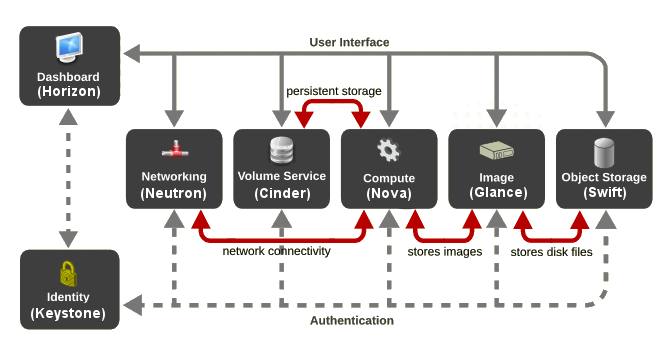
\includegraphics[clip= true, width= \columnwidth]{images/openstack_core_components.png}
	\caption{Internal components interaction.}
	\label{fig:OS_components_interraction_logical}
\end{figure}

\subsubsection{Identity - Keystone}
\label{sec:keystone}
As a distributed environment, the system has to provide secure access and hence both users and services must authenticate themselves before performing any operation.
OpenStack developers wrote a specific service called \textbf{Keystone} for this purpose; it stores username and password for each authorized user/service, the authorization process involves obtaining a token to be used later to perform requests to other services. The general concept behind a token-based authentication system is simple: it allows users to enter their username and password in order to obtain a token, which enables them to fetch a specific resource - without using their username and password again. Once the token has been obtained, the user can use the token, which offers access to a specific resource for a time period. Identity also correlate a user to its role in the system, and the visibility of resources. Administrators are able to see everything that is going on in the system, while a common user can only see the virtual resources he created.
This separation of group belonging in keystone is called role and is used by other services to check whether the user is authorized or not to perform such operation, basically defining a sandbox for each user so that anyone can only see what he is authorized to.
Alongside the user concept, keystone defines three fundamental terms which are group, tenant (or project) and domain; in this way rules can be associated to them instead of directly to a user. These terms are remapped to internal data-types; here below a list of Keystone resources is given alongside with a brief description and usage:
\begin{itemize}
	\item User: contains account credentials and is associated with one or more projects or domains.
	\item Group: a collection of users; it is associated with one or more projects or domains.
	\item Project (Tenant): unit of ownership in OpenStack; it contains one or more users part of a Group.
	\item Domain: contains users, groups and projects.
	\item Role: a piece of metadata associated with many user-project pairs.
	\item Token: identify credential related to a user or to a user-project pair.
	\item Extras: bucket of key-value metadata associated with a user-project pair; it is intended to provide a method to send extra fields in a REST call without changing its interface.
	\item Rule: describes a set of requirements for performing an action.
\end{itemize}
Since credentials are generally built from the user metadata in the \texttt{"extras"} field of the Identity API, adding a \texttt{"role"} to a user just means to add the role to the metadata.
Data-types are used inside keystone to provide a set of services that are exposed to users via one or more HTTP endpoints:
\begin{itemize}
	\item Identity: this service is intended to provide authentication, credential validation and data about Users, Groups, Projects, Domains and Roles, as well as any associated metadata. In the basic case all these data is managed directly by the service itself that exposes all the CRUD methods associated with the data.
	\item Token: service that validates and manages tokens that are used when performing requests, typically to other services; a token is created once a user credentials have been verified.
	\item Catalog: which provides a registry used for endpoint discovery, this permits to know how to contact all the other services.
	\item Policy: this service provides a rule-based authorization engine and the associated rule management interface.
\end{itemize}
Policies based on a set of rules can be specified for each OpenStack component; all components have their own \textit{"policy.json"} file that permits to associate rules to all Openstack service actions. In listing~\ref{lst:nova_policy} is an example of policy.json file of Compute service (Nova) in which is defined - lines 14 and 15 - a policy that only permits to the user identified as the owner or an administrator to start or stop a VM, meaning that someone that shares a project with the previous user is not allowed to manage a VM not belonging to him.
\lstinputlisting[label=lst:nova_policy, language=python, caption={policy.json file relative to the Nova service.}]{code/nova_policy.json}

\begin{comment}
Each one of the Keystone services listed above can potentially be connected to a different backend, this is done to allow Keystone to fit a variety of environments and needs. The most popular choice is a SQL based one that leverages SQLAlchemy to store data persistently. If this solution is adopted, the keystone-manage command can be used to introspect the backend and, by running the \texttt{"db\_sync()"} subcommand, to upgrade the database schema. In substitution to this first classical solution, a Lightweight Directory Access Protocol (LDAP) backend can be used to store users and projects in separate subtrees, roles then are recorded as entries under the projects they belong to. The possibility to choose between different kinds of backend is mainly available thanks to the structure that the majority of OpenStack projects have, that is an abstract class defines basic interactions and primitives callable by frontend services, these functions are then implemented inside a set of special purpose classes, each one dedicated to manage a specific storage system. Administrators can then specify which backend they want and are going to use inserting a proper entry into the dedicated configuration file section.
As well as the backends, OpenStack has a common way to manage the API call and keystone makes no exception. As in other services, an HTTP front-end is exported by using the python WSGI interface. HTTP endpoints are made up of pipelines of WSGI middleware that, in turn, use a subclass called \texttt{"ComposingRouter"} that takes care of linking URLs to one of the defined controllers; within each controller, one or more managers are loaded. Managers are thin wrapper classes in charge of loading the appropriate service driver based on the keystone configuration.
\end{comment}

\subsubsection{Storage - Cinder, Swift and Glance}
\label{sec:openstack_storage}
Numerous projects have been started focusing on different specific purposes related to disk management.

\textbf{Block storage} - known as Cinder - allows to dynamically attach additional disks to virtual machine instances. This ability allows to scale up the available disk size of a specific virtual machine avoiding the need to destroy and recreate the same instance only with more storage space.

\textbf{Object storage} - codename Swift - is meant to manage a distributed, API-accessible storage platform that can be integrated directly into applications or used for backup, archiving and data retention. This comes particularly handy in the typical scenario of a datacenter where the computing power is kept separated from the large hard drives where data reside. Swift provides similar functionalities that a network-attached storage (NAS) does.

Unlike the two above cited services that are not identified as OpenStack core components, the \textbf{image service} (Glance) is very important and provides the ability to retrieve, copy and snapshot a server image and store it leveraging the others storage services or interacting directly with the local file system.
Images can be uploaded in various formats and pinned as public or stay private, meaning that they can be used only by the user that created them.
A service that takes care to allow customers to manage their own base images and create snapshots is crucial to provide a flexible customizable experience to end users.
Glance has a RESTful API that allows querying for snapshot's metadata as well as retrieval of the actual image.
This function is crucial in the moment of instantiation of a virtual machine since at startup time a bootable disk is essential.
Associating information to disk image is also trivial at instantiation time when resources are reserved and assigned to a virtual machine. In this moment is essential to check if the given resource quotas are enough to support the chosen image and therefore make the VM work correctly.

\subsubsection{Computing - Nova}
\label{sec:nova}
The compute part is one of the critical services of OpenStack, being the one that actually makes virtual machine instances run.
It is designed to manage and automate pools of compute resources and can work with widely available virtualization technologies, as well as baremetal and high-performance computing (HPC) configurations.
Given its complexity, this component, in turn, has been divided into submodules, each one in charge of one particular task.
\begin{figure}[h]
	\centering
	% left bottom right top
	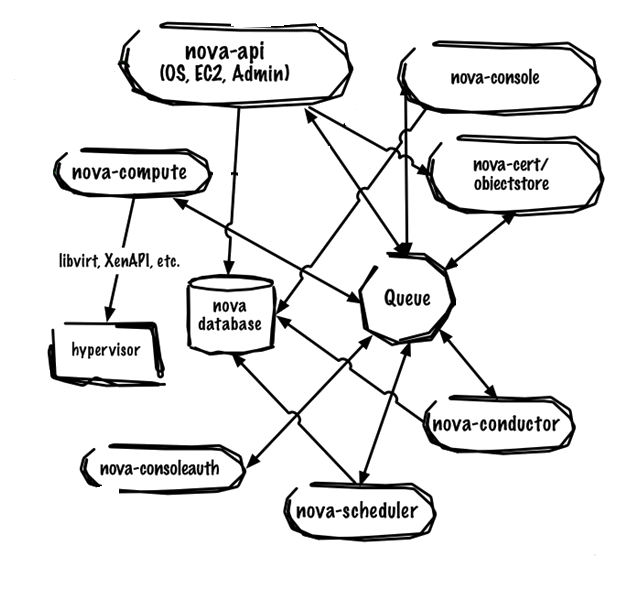
\includegraphics[clip= true, width= 0.6 \columnwidth]{images/nova_components.png}
	\caption{Nova components and interactions.}
	\label{fig:OSnovalogical}
\end{figure}
The two components of particular interest are the compute and the scheduler submodules.
The former is a worker daemon called \textbf{nova-compute} and resides in each compute node. It is in charge of creating and terminating virtual instances through hypervisor APIs, for example XenAPI for XenServer/XCP, VMwareAPI for VMware, libvirt for KVM and others as depicted in Figure~\ref{fig:OSnovacompute}.
Given that KVM and XenServer are popular choices for hypervisor technology and recommended for most use cases, OpenStack also wants to meet the needs of those administrators that do not have at their disposal a large computational power and might want to use a linux container technology such as LXC, and wish to minimize virtualization overhead and achieve greater efficiency and performance. In addition to different hypervisors, OpenStack supports Intel, ARM and other hardware architectures.
The nova-compute agent is also in charge of letting the other nova submodules located in the controller node aware of its existence and status, this job is done by sending periodical messages to the message broker service.
\begin{figure}[h]
	\centering
	% left bottom right top
	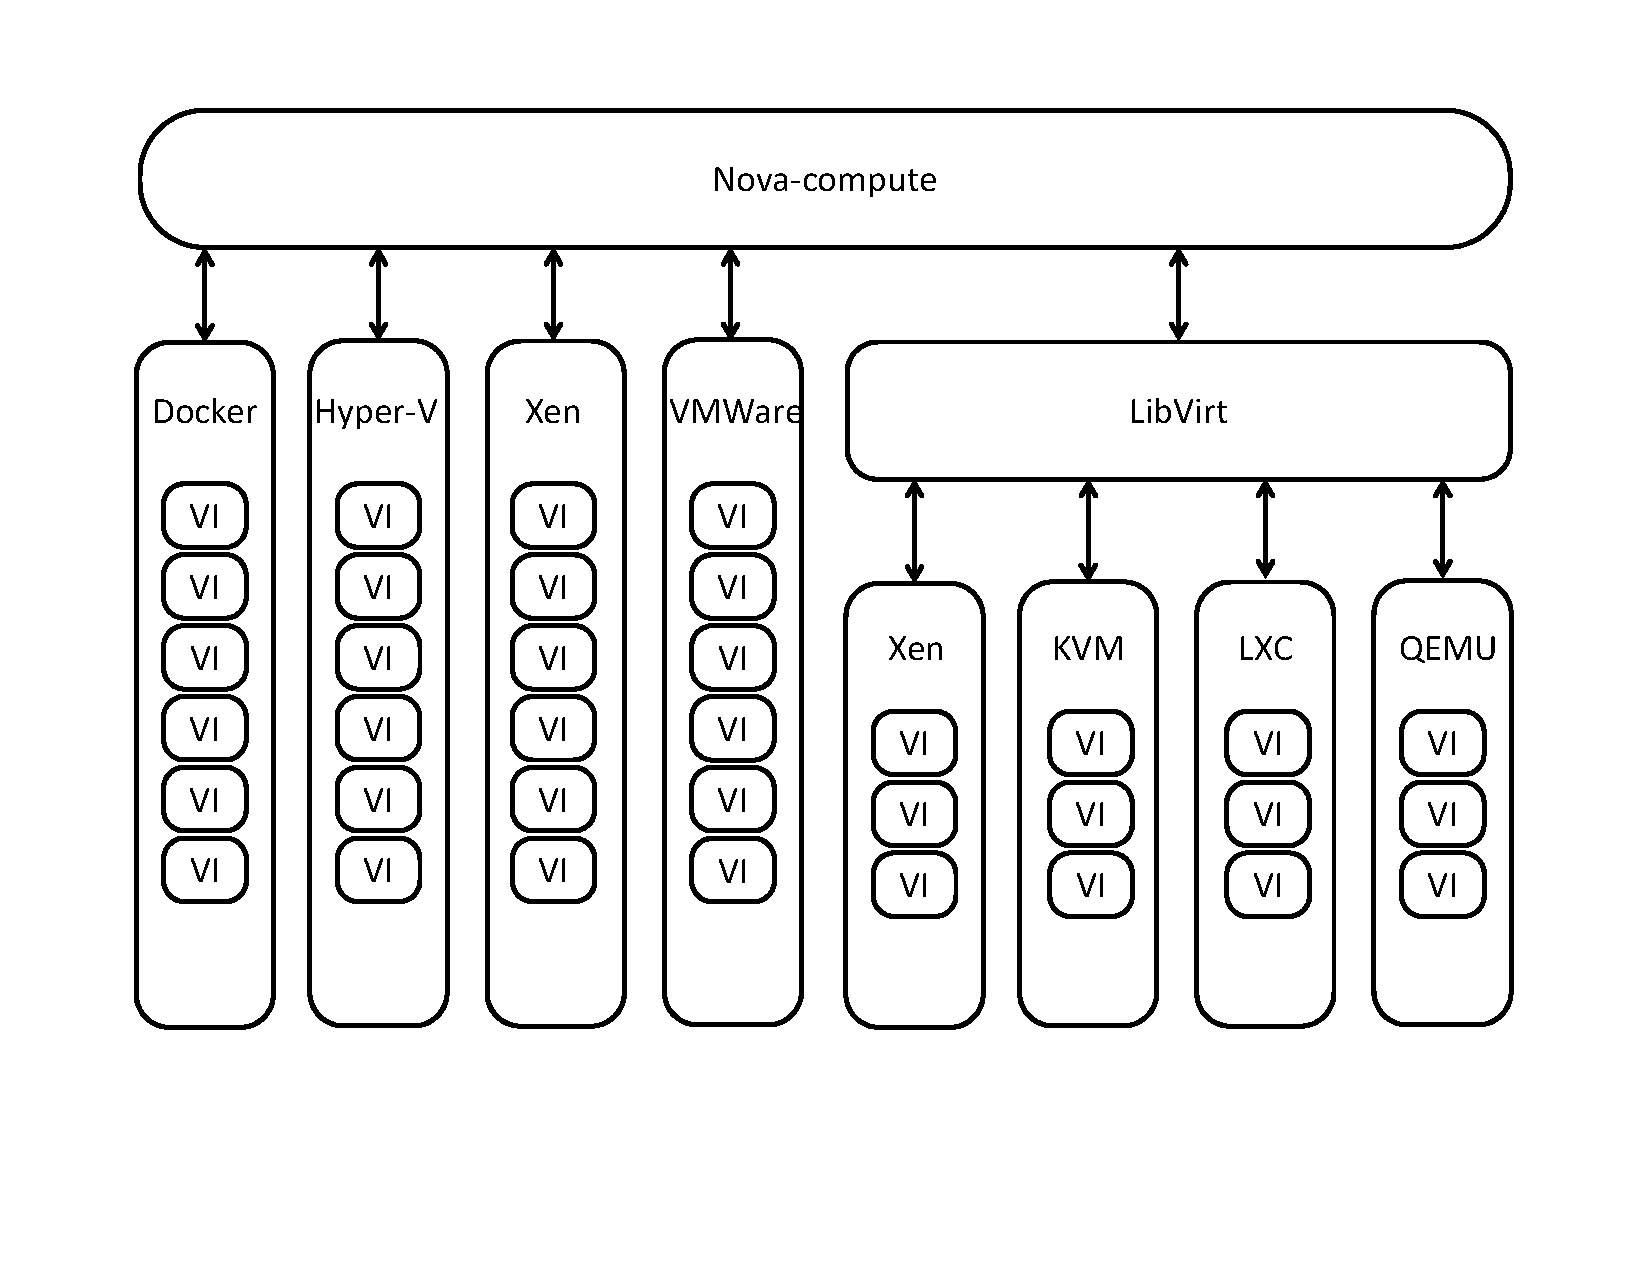
\includegraphics[clip= true, width=0.8 \columnwidth]{images/nova-compute.pdf}
	\caption{Nova compute hypervisors support.}
	\label{fig:OSnovacompute}
\end{figure}
In the controller node are located both the module that manages requests (\textbf{nova-api}) and the \textbf{nova-scheduler}, which is in charge of choosing where the virtual machines are going to be instantiated.
The scheduler submodule is very important and valuable for an administrator that wants to maximize the efficiency of the entire system.
As default, OpenStack comes with an algorithm that takes decisions in a two-steps process called filter and weight, a representation of this sequence of events is given in Figure~\ref{fig:OSnovascheduler}.
In the first step, it excludes from all the available hosts, the ones that do not meet specific requirements (e.g., free resources, architecture, hypervisor, etc), while in the second step all feasible hosts remained after the filtering are weighed according to a predefined cost function. The filter manager module is explicitly thought in a way that new constraints can be defined to further skim the pickable nova-compute module.
On the contrary of the filter module, the weighing function is customizable but unique so it has to be tuned with consciousness; its only purpose is to model each remaining host with a number, then the host with the highest value is chosen and the command to instantiate the virtual machine is dispatched to the corresponding nova-compute agent.
Both filter and weight steps take into consideration the information - generally referred as host status - exported by each nova-compute that typically consists in free resource availability.
\begin{figure}[h]
	\centering
	% left bottom right top
	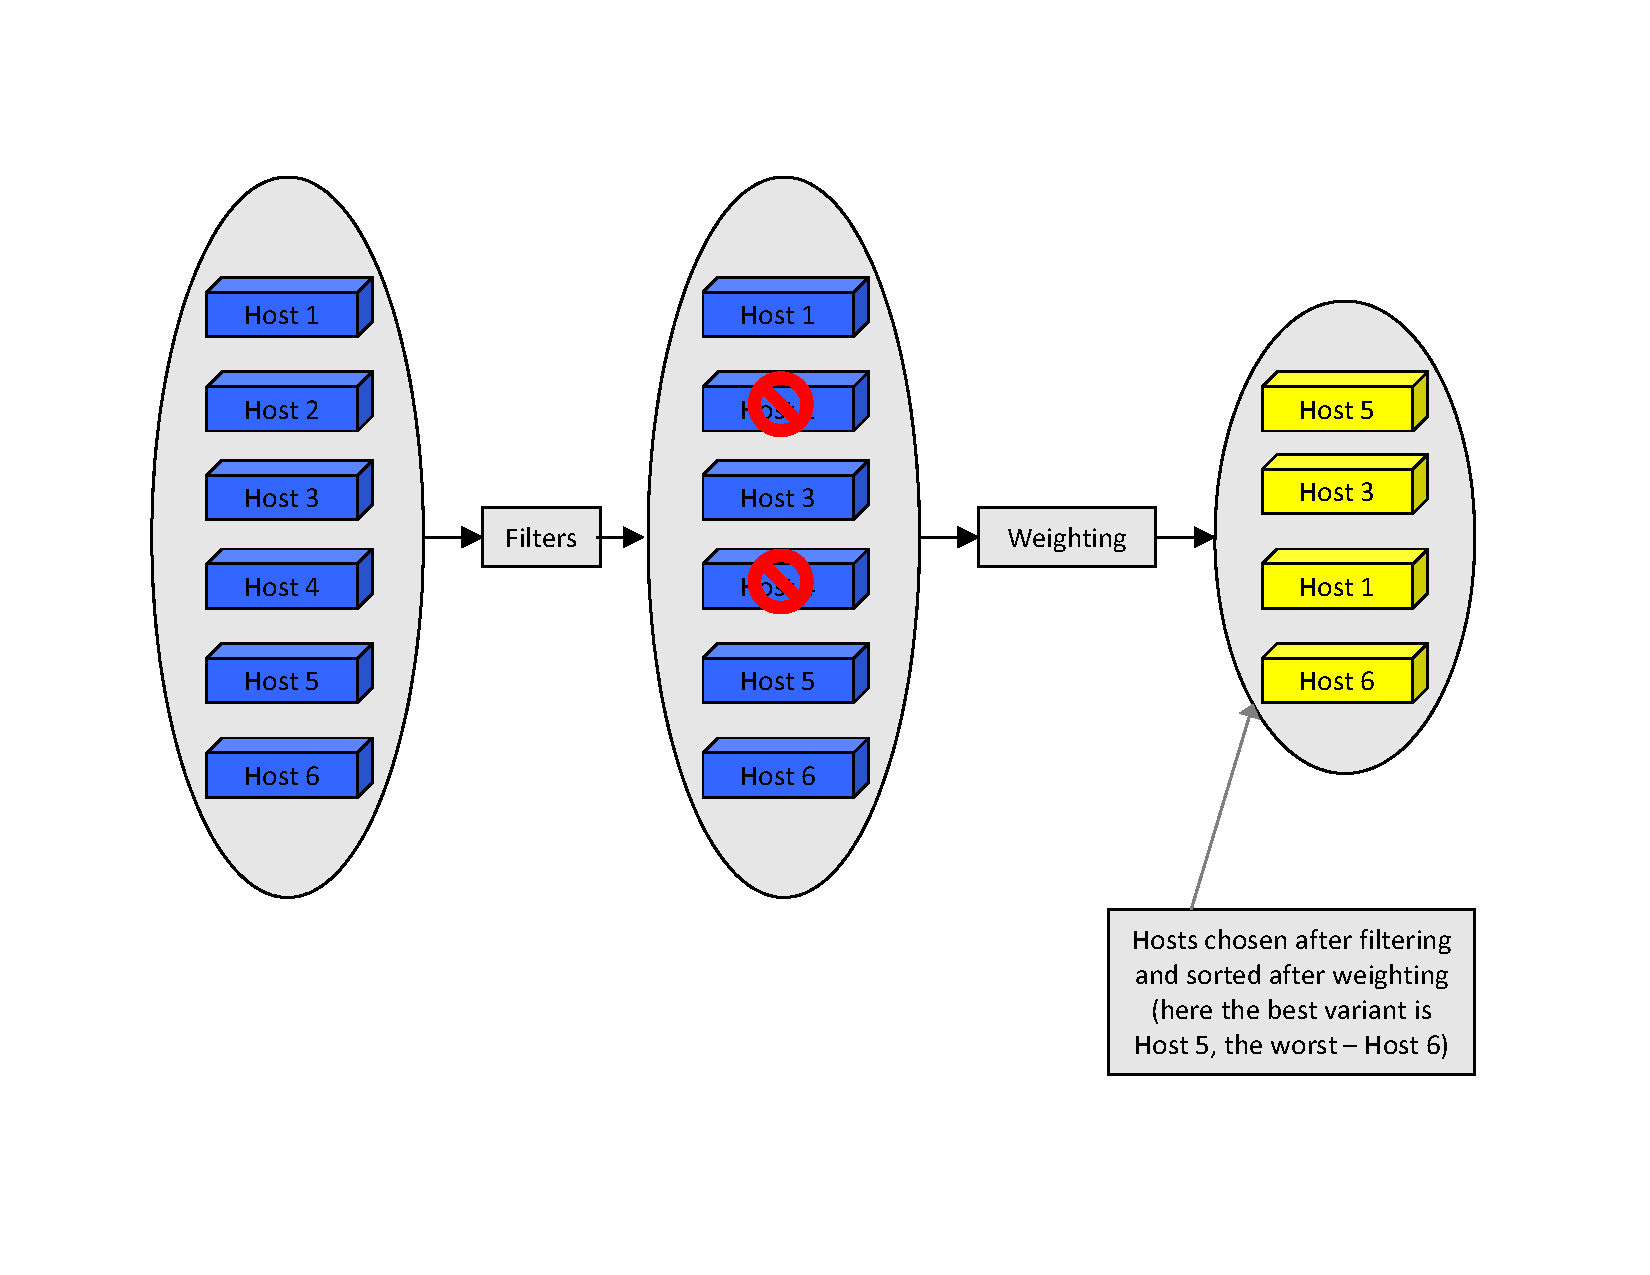
\includegraphics[clip= true, width= \columnwidth, trim=0cm 3cm 0cm 3cm]{images/nova-filter-weight.pdf}
	\caption{Filter and weight scheduling process.}
	\label{fig:OSnovascheduler}
\end{figure}

\subsubsection{Network - Neutron}
\label{sec:neutron}
As well as Nova, \textbf{Neutron} is also a core component of OpenStack and it is in charge of managing the network that interconnects the virtual machines.
Actually, it would be more correct to say that it is in charge of managing the virtual overlay network that interconnects the virtual machines as it does not have any knowledge about the physical interconnections between compute nodes.
Neutron, formerly known as Quantum, provides users an abstraction that allow them to interconnect their own virtual machines and define some basic network services such as router, dynamic host configuration protocol (DHCP), firewall and virtual private network (VPN) terminator, decide which IP address assign to a VM and choose whether a VM is reachable from the Internet or not.
When a user decides to modify his own network topology or performs operations such as launching or stopping a virtual machine, Neutron quickly reconfigures the virtual switches - br-int, br-tun/br-net - to provide connectivity and isolation.
In order to understand the level of abstraction provided by this component, it is necessary to look at the network at three different levels.
First comes the lower layer, composed of the physical equipments such as Ethernet cables, optical fibers and hardware switches; on top of this, a full mesh of generic routing encapsulation (GRE) tunnels are established between all the br-tun/br-net virtual switches infrastructure explained in section \ref{a:br_section}.
Over this layer lays the actual user defined networks, modeled with virtual local area network (VLAN) and carrying the traffic through the GRE tunnels.
This behavior is modifiable by intervening on the configuration files of Neutron and therefore adapting this service to better suits the datacenter communication infrastructure.
Being this flexible requires Neutron to have a structure as the one in Figure~\ref{fig:neutron_structure}, where five levels are indicated.
\begin{figure}[h]
	\centering
	% left bottom right top
	\includegraphics[clip= true, width= \columnwidth, page=53, trim=0cm 8cm 0cm 0cm ]{images/Pictures_definitivo.pdf}
	\caption{Neutron architecture.}
	\label{fig:neutron_structure}
\end{figure}
The first two from the top are in charge of receiving requests, serialize and transform them into objects that models Neutron resources. The user is provided with a set of primitive to create his own network topology; these primitives are nothing less than Neutron resources that are:
\begin{itemize}
\label{neutronresourcelist}
    \item Network - defines a L2 broadcast domain.
    \item Subnet - in a network, it defines an IP address range
    \item Port - in a subnet, it defines an attachment point for either a VM, a router or a firewall.
\end{itemize}
Scrolling down the architectural stack (shown in figure~\ref{fig:neutron_structure}), there is the Modular Layer 2 plug-in (ML2), which is in charge of keeping the internal status of the network service to provide robustness and recoverability after a major failure of the neutron component. It also fulfill the \texttt{"GET"} requests that are useful for example to the dashboard to represent in a graphical manner all the information relative to the user's network topology.
Below the ML2 there are two managers layer that are in charge of dispatching requests to type and mechanism driver modules.
Both the drivers kind are intended to provide and implement per user and - if required - per user's network isolation. Let's say that the type driver decides the standard that is going to be used and the mechanism is in charge of implementing it.
Type drivers are pluggable modules in which information about how to guarantee isolation are added to the Neutron objects. The modified object is then returned to the third level of the stack that finally passes it to the other manager which is in charge of dispatching the received object to one or more drivers.
A mechanism driver is specifically designed to communicate with a particular virtual switch that resides in the compute nodes. This component is crucial and each vendor can easily develop one that remaps Neutron objects (listed in~\ref{neutronresourcelist}) to commands specific to its device; OpenStack comes with already a lot of drivers from which to choose; for example the one for openvswitch, linuxbridge and the one developed expressly for the integration with OpenDaylight which will be described in section \ref{sec:opendaylight}.
Mechanism drivers are actually called twice each time a resource is created, updated or deleted: before the ML2 database operation and then again after that the data-base transaction is concluded successfully.
This double call allows to the mechanism driver to prepare and check the feasibility of the operation and only after it the grant from the upper layer, the operation is actually performed.
To summarize, Neutron other than providing connectivity between VMs, also establishes user isolation in a way that inter-user communication can happen only via a public network defined by the administrator for this specific purpose.

\subsubsection{Orchestration - Heat}
\textbf{Heat} is the main project in the OpenStack Orchestration program. It implements an engine to launch multiple composite cloud applications based on templates in the form of text files that can be treated like code. It aims to export a unique-common API usable by the user to instantiate a complete network topology comprehensive of virtual machines in the form of a template making just one call; the Heat engine then takes care of translating such template into calls for both Nova and Neutron. In order to improve performance, all these calls will be made in parallel unless dependencies between resources are implicitly or explicitly specified. As an example of implicit dependency let's consider neutron resources listed in \ref{neutronresourcelist}: a Neutron port attached to a network can exist only if that specific network has already been created.
On the other hand, as explicit dependence the user can point out that a virtual machine must be created before another one - a valid motif can be that the first VM provides services without which the second one cannot boot correctly.
Another useful feature is the management of updates.
When a request is received by Heat and it contains a reference to an already instantiated template, the engine is able to understand what is changed between the allocated resources and the ones present in the request - this is done similarly to the \texttt{"diff"} unix/linux command.
Once this task has come to an end, the creation, modification and/or deletion of resources will be handled; the new ones will be created and the no more needed can be deleted.
For what concerns the update of a resource, Heat allows two ways of behavior. The first one is to rawly destroy the elder and then create a new one with the up-to-date characteristics. A more sophisticated approach is to define in each service the way to handle the update locally (e.g., change the static ip address of a port), however this is not always possible - an example is the case of changing the disk image of a VM.

\subsubsection{Dashboard - Horizon}
Usability is essential in complex systems, hence programmers typically offer a user friendly interface, avoiding the unexperienced users the pain of going through a complex command line tool.
Under this aspect, OpenStack is not an exception and provides a well structured web dashboard called Horizon, from which administrators can monitor the system and users can easily perform operations that otherwise require a long list of command-line inputs.
The dashboard follows the OpenStack's main concept of abstraction and models VMs, networks and network services in a way that even an unexperienced user can easily understand. In Figure~\ref{fig:OSdashboard} is given a screen-shot of what a user sees when a simple topology is deployed. As is evident from the image, there is no indication about the physical location of the VMs (VM1, VM2, VM3), the service (Router) and other user instances.
\begin{figure}[h]
	\centering
	% left bottom right top
	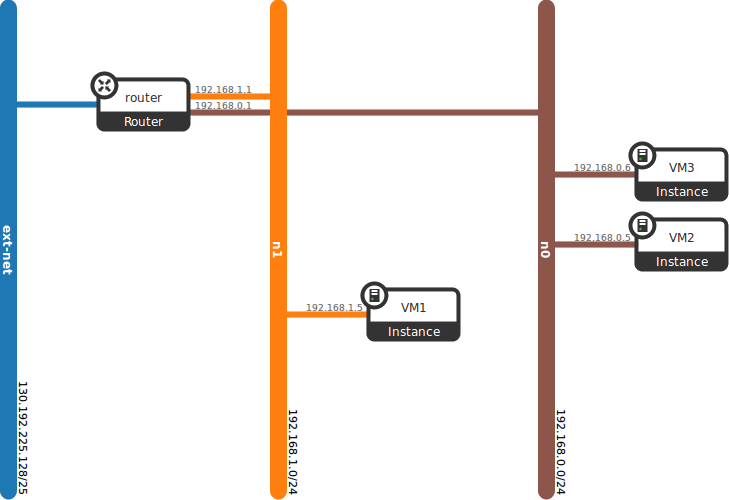
\includegraphics[clip= true, width=0.9 \columnwidth]{images/neutron-topology-example.png}
	\caption{Dashboard view of network topology design with VMs.}
	\label{fig:OSdashboard}
\end{figure}

\subsubsection{Command line clients}
Since all services are meant to receive commands via REST API, OpenStack developers have produced a command-line based client for each project that automates otherwise pedantic operation and complex typing of unicode strings.
These clients perform a series of cURL requests to obtain the required result.
As an example, consider that a user that wants a list of all his virtual machines with some details, using the client, it is easy: just type \texttt{"nova list"}. To achieve the same result, it is mandatory to acquire an authentication token, then use it to query the nova-api and obtain the list of instances. If more details are required, a request for each machine has to be dispatched.
Other than automation, clients provide also data presentation so that instead of receiving responses in form of raw JSON or XML, better-looking and compact tables are displayed.

\subsection{OpenStack towards NFV}
The OpenStack community continues to grow and the number of companies that decide to adopt the open-source solution is constantly augmenting. As it is easy to imagine, these companies work in different fields and have various needs. Keep up with all the requests of new features implementations is almost impossible but the community does its best to at least try. In this optic a new squad, called NFV team, is trying to propose new solutions that should be integrated into OpenStack to better support network function virtualization.
As stated in their official page\cite{NFVteam}, their mission aims to define the use cases, identify and prioritize the requirements that are needed to run Network Function Virtualization workloads on top of OpenStack. This work includes identifying functional gaps, creating blueprints, submitting and reviewing patches to the relevant OpenStack projects and tracking their completion in support of NFV. The requirements expressed by this group should be made so that each of them have a test case which can be verified using an open-source implementation. This ensures that tests can be done without any special hardware or proprietary software, which is key for continuous integration tests in the OpenStack gate. If special setups are required which cannot be reproduced on the standard OpenStack gate, the use cases proponent will have to provide a 3rd party CI setup, accessible by OpenStack infra, which will be used to validate developments against. All the proposals they have ever made can be found on their website\cite{NFVteam} along with their statuses. Looking at the number of active blueprints it can be seen that as a group they are very active so there is quite the possibility their work towards a NFV fully-capable OpenStack will lead to nice results. As a down side, each one of their proposition has to be discussed, reviewed,validated, implemented and finally tested. It is evident that such procedure requires time, also it has to be compatible with all the already existent features.
As an example, let's take the \textit{Services Insertion, Chaining and Steering}\cite{neutronsteeringofficial} extension they proposed for the neutron module. Taking a look at the white-board it can be easily seen the time it is required to finally come to a working implementation; in fact it the proposal came up on late 2013 and as far as October, the 13th 2014 this project still has not been marked as approved.
Even if its purpose is quite similar to the FlowRule abstraction, this proposed extension has evolved during the year coming to look more like the ETSI service chain instead of appearing like an OpenFlow rule as the FlowRule does.
Instead of defining a port-to-port connection with matching rules, they decided to introduce two kinds of resources: \textit{ports chain} and \textit{label}.
A label is no more than a series of OpenFlow-like fields that will identify a traffic flow. Consequently a set of neutron ports are ordinately grouped to create a ports chain.
Finally a ports chain can be associated to a label; in this way all the information to perform traffic steering are provided to neutron.
With the wisdom of hindsight this approach looks more elegant than the one introduced by us; it has to be said though that our extension, (with all its limits) have been implemented in just few weeks. Furthermore, being an ad-hoc design, is able to support traffic steering between ports that are not been instantiated by OpenStack, permitting to bypass the limitations imposed by the network node (e.g., obligation for the traffic incoming and outgoing to pass through the virtual router).
Taking another look at the NFV team's blueprint list, we can find a set of interesting proposals from which our architecture can benefit. As an example there are the \textit{unaddressed interfaces for NFV use cases} that brings up the idea of defining transparent ports and this is precisely our use case.
Furthermore they also have numerous blueprints that aim to improve the nova scheduler, unfortunately no one focused toward a network aware scheduling.

\section{OpenDaylight}
\label{sec:opendaylight}
OpenDaylight (ODL), as presented in the official project website\cite{Opendaylightwebsite}, is an open platform for network programmability to enable SDN and NFV for networks.
The software is a combination of components including a fully pluggable controller, interfaces, protocol plug-ins and applications. With this common platform both customers and vendors can innovate and collaborate in order to commercialize SDN and NFV based solutions.
If stripped to its very minimal core, it results to be just an openflow controller, which is able to instruct the controlled switches to behave in a certain way.
There are numerous openflow controller projects since the standard came out back in December 2009 but there are factors that really differs OpenDaylight from the others; first there is the community that keeps developing it, some major vendors such as Cisco, IBM, HP, Brocade Juniper, Microsoft and others also support the project both economically and with workforce.
Secondly it has been engineered to make easy for developers to add their additions in form of a bundle that will easily integrate and interact with the core components and other plug-ins either available in the public repository, proprietary or created by other developers.

\section{Integration between the two projects}
Already in the first official stable release of OpenDaylight - codename Hydrogen - published in February 2014 and in particular in the \texttt{virtualization} version, a plug-in for the integration with OpenStack was made available. This add-on represent the first step towards what will likely become the de facto standard for datacenters management. Being in its early times, the OpenDaylight framework and therefore the functionalities exported to OpenStack Neutron, the behavior is sometimes different from the expected one; either way making this two software products work together in a cooperative way is an aspect of particular interest. In fact as mentioned before OpenStack sees the entire underlaying physical network as a commodity and has no control over it, OpenDaylight on the other hand has been projected to do exactly so.
The integration between the two projects will result with the possibility to aggregate the full control of the datacenter in the aspects of both managing the compute and tuning the network accordingly in an automated and robust way with lot of space for improvement and optimization of performance and capabilities resulting in a better quality of service (QoS), lower management cost and even in the chance of offering users new custom functionalities.
However leveraging these functionalities requires an OpenDaylight fully controlled network and in order to allow that the whole datacenter communication system needs to be openflow-capable.
Given that openflow physical switches are still not so common on the market, having the possibility to pilot them with the very same controller that manages the virtual switches in the compute nodes will be an enormous plus for the datacenter network administrators whom will be allowed to control, configure and monitor all the devices from a unique and centralized point.
